

\PassOptionsToPackage{unicode=true}{hyperref} % options for packages loaded elsewhere
\PassOptionsToPackage{hyphens}{url}
\PassOptionsToPackage{dvipsnames,svgnames*,x11names*}{xcolor}
%
\documentclass[]{book}
\usepackage{lmodern}
\usepackage{amssymb,amsmath}
\usepackage{ifxetex,ifluatex}
\usepackage{fixltx2e} % provides \textsubscript
\ifnum 0\ifxetex 1\fi\ifluatex 1\fi=0 % if pdftex
  \usepackage[T1]{fontenc}
  \usepackage[utf8]{inputenc}
  \usepackage{textcomp} % provides euro and other symbols
\else % if luatex or xelatex
  \usepackage{unicode-math}
  \defaultfontfeatures{Ligatures=TeX,Scale=MatchLowercase}
\fi
% use upquote if available, for straight quotes in verbatim environments
\IfFileExists{upquote.sty}{\usepackage{upquote}}{}
% use microtype if available
\IfFileExists{microtype.sty}{%
\usepackage[]{microtype}
\UseMicrotypeSet[protrusion]{basicmath} % disable protrusion for tt fonts
}{}
\IfFileExists{parskip.sty}{%
\usepackage{parskip}
}{% else
\setlength{\parindent}{0pt}
\setlength{\parskip}{6pt plus 2pt minus 1pt}
}
\usepackage{xcolor}
\usepackage{hyperref}
\hypersetup{
            pdftitle={The Open Quant Live Book},
            pdfauthor={Thársis T. P. Souza},
            colorlinks=true,
            linkcolor=Maroon,
            filecolor=Maroon,
            citecolor=Blue,
            urlcolor=Blue,
            breaklinks=true}
\urlstyle{same}  % don't use monospace font for urls
\usepackage{geometry}
\geometry{paperwidth=6in, paperheight=9in}
\usepackage{color}
\usepackage{fancyvrb}
\newcommand{\VerbBar}{|}
\newcommand{\VERB}{\Verb[commandchars=\\\{\}]}
\DefineVerbatimEnvironment{Highlighting}{Verbatim}{commandchars=\\\{\}}
% Add ',fontsize=\small' for more characters per line
\usepackage{framed}
\definecolor{shadecolor}{RGB}{248,248,248}
\newenvironment{Shaded}{\begin{snugshade}}{\end{snugshade}}
\newcommand{\KeywordTok}[1]{\textcolor[rgb]{0.13,0.29,0.53}{\textbf{#1}}}
\newcommand{\DataTypeTok}[1]{\textcolor[rgb]{0.13,0.29,0.53}{#1}}
\newcommand{\DecValTok}[1]{\textcolor[rgb]{0.00,0.00,0.81}{#1}}
\newcommand{\BaseNTok}[1]{\textcolor[rgb]{0.00,0.00,0.81}{#1}}
\newcommand{\FloatTok}[1]{\textcolor[rgb]{0.00,0.00,0.81}{#1}}
\newcommand{\ConstantTok}[1]{\textcolor[rgb]{0.00,0.00,0.00}{#1}}
\newcommand{\CharTok}[1]{\textcolor[rgb]{0.31,0.60,0.02}{#1}}
\newcommand{\SpecialCharTok}[1]{\textcolor[rgb]{0.00,0.00,0.00}{#1}}
\newcommand{\StringTok}[1]{\textcolor[rgb]{0.31,0.60,0.02}{#1}}
\newcommand{\VerbatimStringTok}[1]{\textcolor[rgb]{0.31,0.60,0.02}{#1}}
\newcommand{\SpecialStringTok}[1]{\textcolor[rgb]{0.31,0.60,0.02}{#1}}
\newcommand{\ImportTok}[1]{#1}
\newcommand{\CommentTok}[1]{\textcolor[rgb]{0.56,0.35,0.01}{\textit{#1}}}
\newcommand{\DocumentationTok}[1]{\textcolor[rgb]{0.56,0.35,0.01}{\textbf{\textit{#1}}}}
\newcommand{\AnnotationTok}[1]{\textcolor[rgb]{0.56,0.35,0.01}{\textbf{\textit{#1}}}}
\newcommand{\CommentVarTok}[1]{\textcolor[rgb]{0.56,0.35,0.01}{\textbf{\textit{#1}}}}
\newcommand{\OtherTok}[1]{\textcolor[rgb]{0.56,0.35,0.01}{#1}}
\newcommand{\FunctionTok}[1]{\textcolor[rgb]{0.00,0.00,0.00}{#1}}
\newcommand{\VariableTok}[1]{\textcolor[rgb]{0.00,0.00,0.00}{#1}}
\newcommand{\ControlFlowTok}[1]{\textcolor[rgb]{0.13,0.29,0.53}{\textbf{#1}}}
\newcommand{\OperatorTok}[1]{\textcolor[rgb]{0.81,0.36,0.00}{\textbf{#1}}}
\newcommand{\BuiltInTok}[1]{#1}
\newcommand{\ExtensionTok}[1]{#1}
\newcommand{\PreprocessorTok}[1]{\textcolor[rgb]{0.56,0.35,0.01}{\textit{#1}}}
\newcommand{\AttributeTok}[1]{\textcolor[rgb]{0.77,0.63,0.00}{#1}}
\newcommand{\RegionMarkerTok}[1]{#1}
\newcommand{\InformationTok}[1]{\textcolor[rgb]{0.56,0.35,0.01}{\textbf{\textit{#1}}}}
\newcommand{\WarningTok}[1]{\textcolor[rgb]{0.56,0.35,0.01}{\textbf{\textit{#1}}}}
\newcommand{\AlertTok}[1]{\textcolor[rgb]{0.94,0.16,0.16}{#1}}
\newcommand{\ErrorTok}[1]{\textcolor[rgb]{0.64,0.00,0.00}{\textbf{#1}}}
\newcommand{\NormalTok}[1]{#1}
\usepackage{longtable,booktabs}
% Fix footnotes in tables (requires footnote package)
\IfFileExists{footnote.sty}{\usepackage{footnote}\makesavenoteenv{longtable}}{}
\usepackage{graphicx,grffile}
\makeatletter
\def\maxwidth{\ifdim\Gin@nat@width>\linewidth\linewidth\else\Gin@nat@width\fi}
\def\maxheight{\ifdim\Gin@nat@height>\textheight\textheight\else\Gin@nat@height\fi}
\makeatother
% Scale images if necessary, so that they will not overflow the page
% margins by default, and it is still possible to overwrite the defaults
% using explicit options in \includegraphics[width, height, ...]{}
\setkeys{Gin}{width=\maxwidth,height=\maxheight,keepaspectratio}
% Make links footnotes instead of hotlinks:
\DeclareRobustCommand{\href}[2]{#2\footnote{\url{#1}}}
\setlength{\emergencystretch}{3em}  % prevent overfull lines
\providecommand{\tightlist}{%
  \setlength{\itemsep}{0pt}\setlength{\parskip}{0pt}}
\setcounter{secnumdepth}{5}
% Redefines (sub)paragraphs to behave more like sections
\ifx\paragraph\undefined\else
\let\oldparagraph\paragraph
\renewcommand{\paragraph}[1]{\oldparagraph{#1}\mbox{}}
\fi
\ifx\subparagraph\undefined\else
\let\oldsubparagraph\subparagraph
\renewcommand{\subparagraph}[1]{\oldsubparagraph{#1}\mbox{}}
\fi

% set default figure placement to htbp
\makeatletter
\def\fps@figure{htbp}
\makeatother

\usepackage{booktabs}
\usepackage{amsthm}
\usepackage{pdfpages}
\usepackage{graphicx}
\usepackage[]{natbib}
\bibliographystyle{apalike}

\title{The Open Quant Live Book}
\author{Thársis T. P. Souza}
\date{2018-12-28}

\let\BeginKnitrBlock\begin \let\EndKnitrBlock\end
\begin{document}

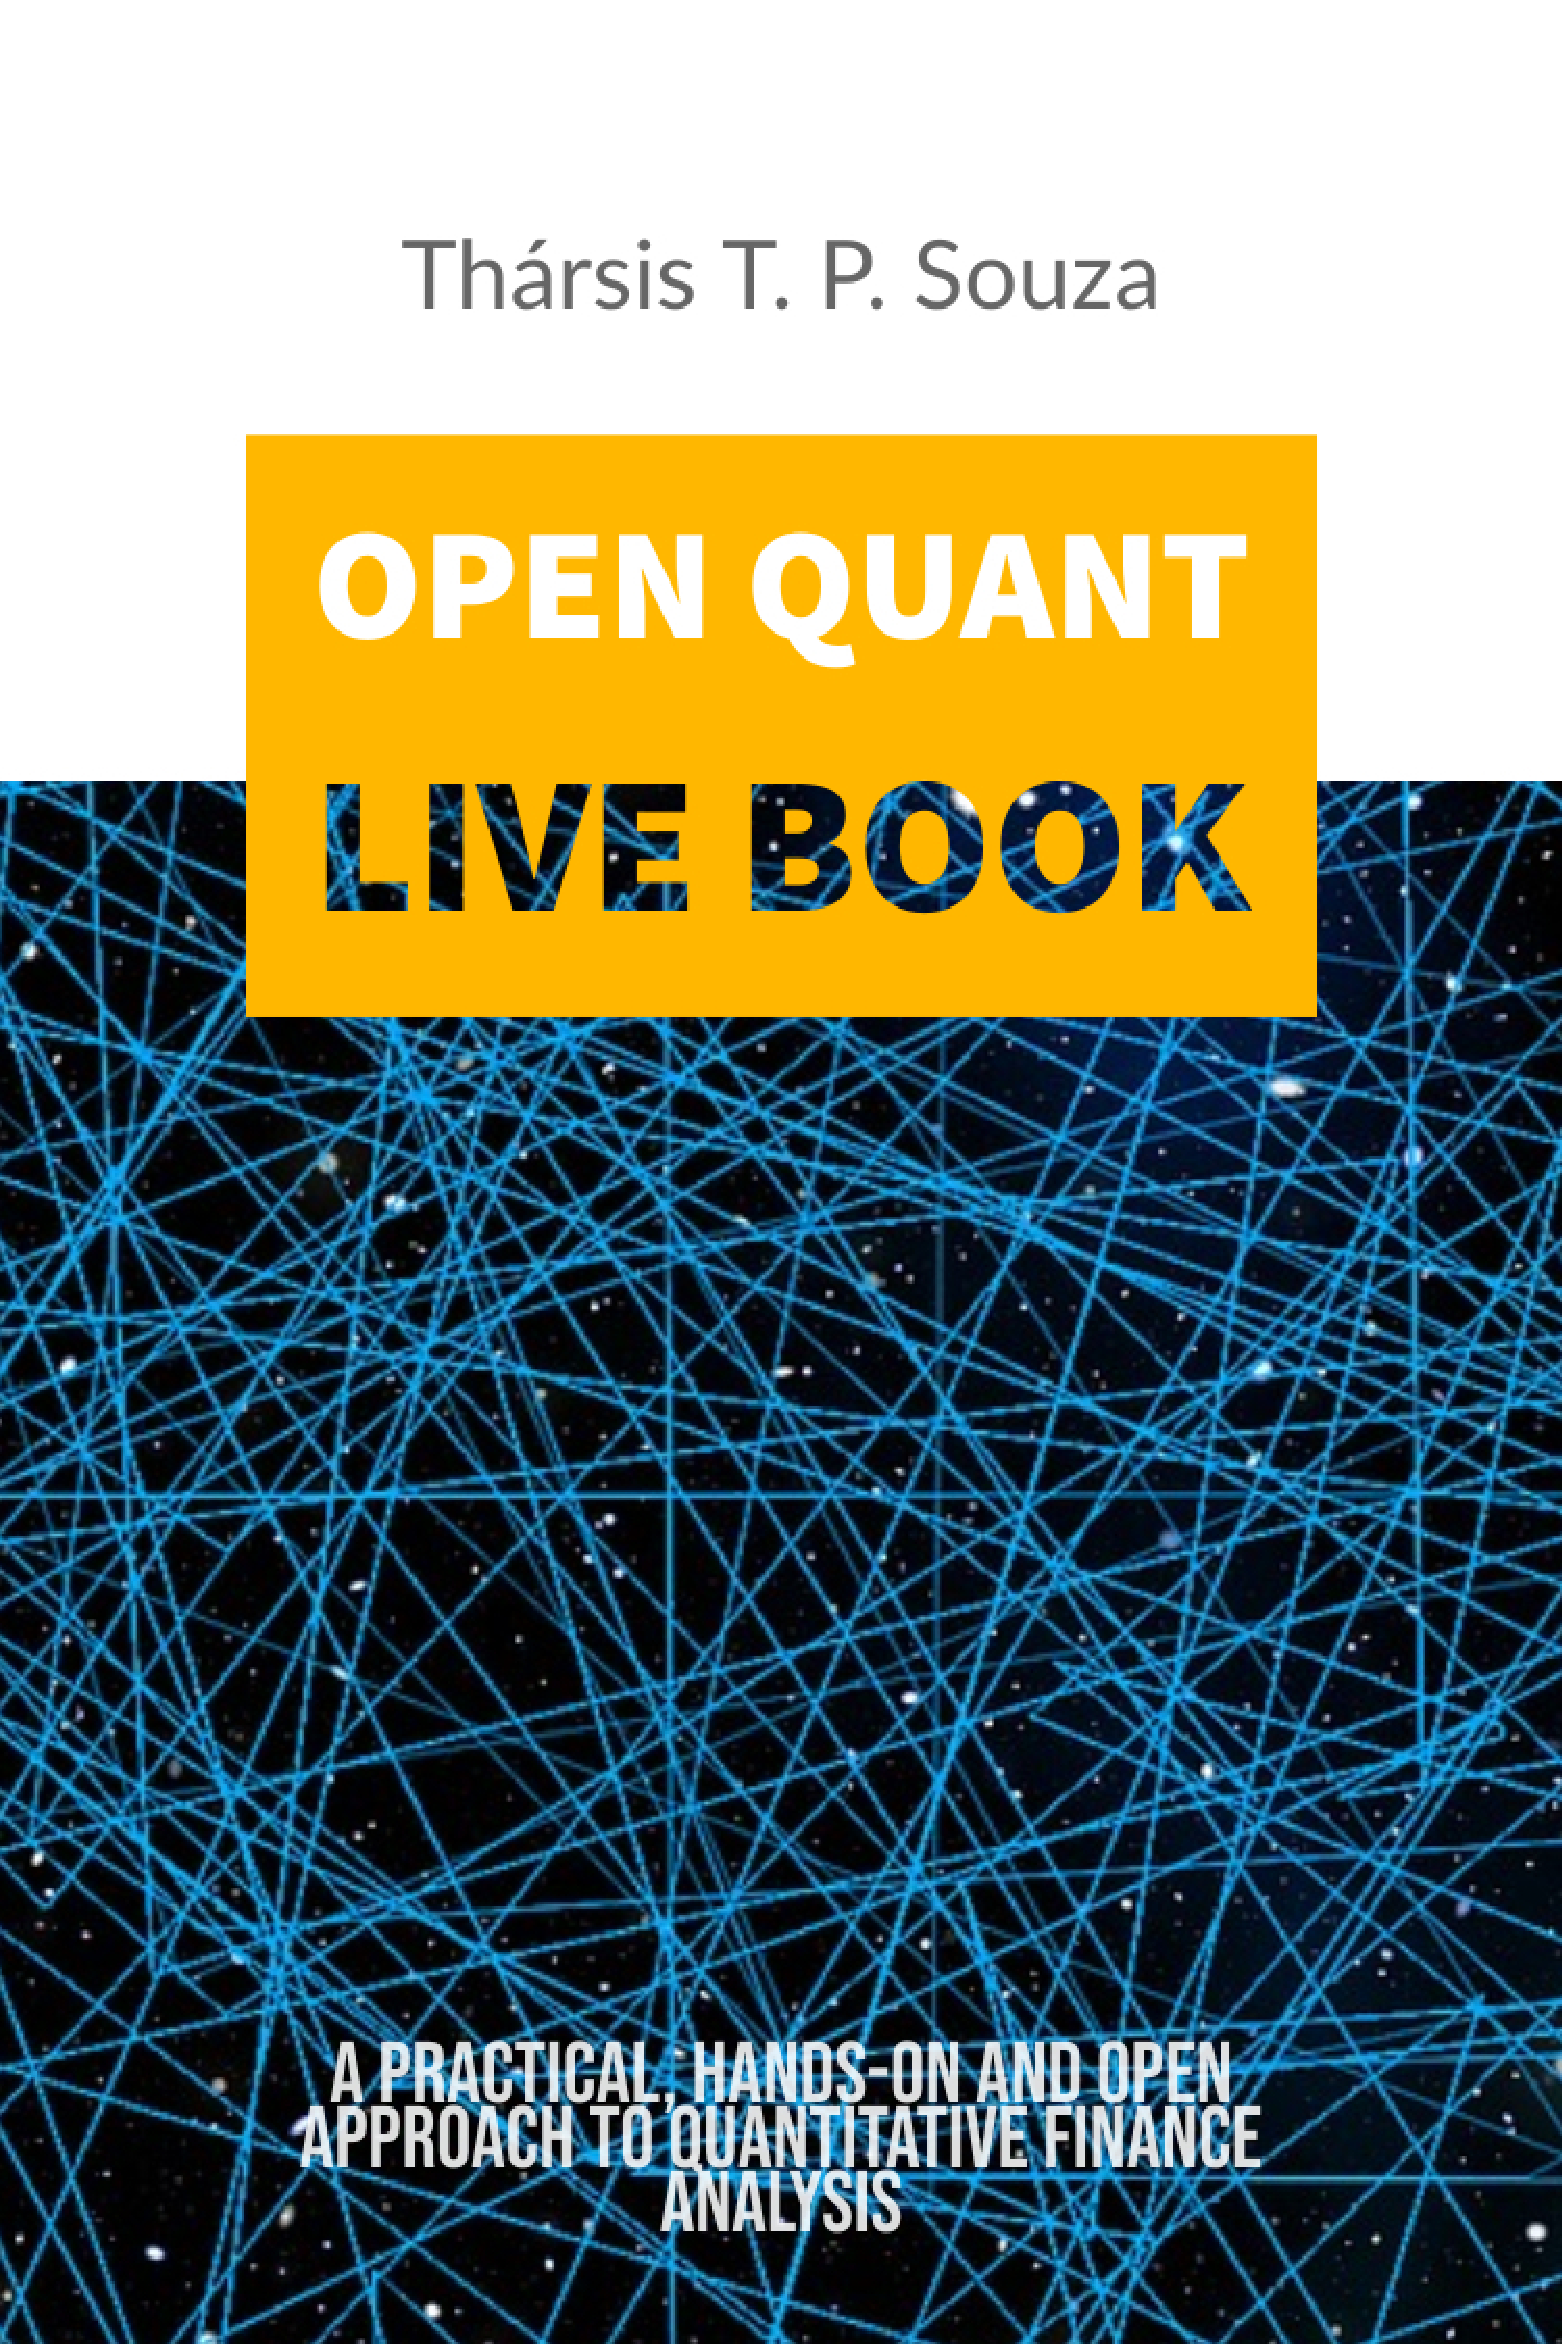
\includepdf{./fig/cover1.pdf}

\maketitle

{
\hypersetup{linkcolor=}
\setcounter{tocdepth}{1}
\tableofcontents
}
\chapter*{Preface}\label{preface}
\addcontentsline{toc}{chapter}{Preface}

\subsection*{Working Contents}\label{working-contents}
\addcontentsline{toc}{subsection}{Working Contents}

\begin{enumerate}
\def\labelenumi{\arabic{enumi}.}
\tightlist
\item
  The Basics
\end{enumerate}

\begin{itemize}
\tightlist
\item
  I/O (25\%)
\item
  Stylized Facts (25\%)
\item
  Correlation \& Causation
\end{itemize}

\begin{enumerate}
\def\labelenumi{\arabic{enumi}.}
\setcounter{enumi}{1}
\tightlist
\item
  Algo Trading
\end{enumerate}

\begin{itemize}
\tightlist
\item
  Investment Process
\item
  Backtesting
\item
  Factor Investing
\item
  Limit Order
\end{itemize}

\begin{enumerate}
\def\labelenumi{\arabic{enumi}.}
\setcounter{enumi}{2}
\item
  Portfolio Optimization
\item
  Machine Learning
\end{enumerate}

\begin{itemize}
\tightlist
\item
  Intro
\item
  AutoML
\item
  Hierarchical Risk Parity
\end{itemize}

\begin{enumerate}
\def\labelenumi{\arabic{enumi}.}
\setcounter{enumi}{4}
\tightlist
\item
  Econophysics
\end{enumerate}

\begin{itemize}
\tightlist
\item
  Entropy, Efficiency and Coupling
\item
  Transfer Entropy, Information Transfer and Causality
\item
  Financial Networks, Taxonomy and Core-Periphery Structure
\end{itemize}

\subsection*{Book's information}\label{books-information}
\addcontentsline{toc}{subsection}{Book's information}

First published at:
\href{https://openquant.netlify.com/}{openquant.netlify.com}.

Licensed under
\href{https://creativecommons.org/licenses/by-nc-sa/4.0/}{Attribution-NonCommercial-ShareAlike
4.0 International}.


\includegraphics[width=0.2\linewidth]{fig/by-nc-sa}

\BeginKnitrBlock{flushright}
Copyright (c) 2018. Thársis T. P. Souza. New York, NY.
\EndKnitrBlock{flushright}

\subsection*{Contribute}\label{contribute}
\addcontentsline{toc}{subsection}{Contribute}

The Book is
\href{https://github.com/souzatharsis/open-quant-live-book}{Open} and we
are looking for co-authors (as I will never have the time or the
knowledge to write it all by myself). Feel free to reach out or simply
create a pull request with your Chapter on our
\href{https://github.com/souzatharsis/open-quant-live-book}{Github
project}.

\part{The Basics}\label{part-the-basics}

\chapter{I/O}\label{io}

\section{Data Sources}\label{data-sources}

\subsection{Alpha Vantage}\label{alpha-vantage}

Alpha Vantage offers free access to pricing data including:

\begin{itemize}
\tightlist
\item
  Stock Time Series Data;
\item
  Physical and Digital/Crypto Currencies (e.g., Bitcoin);
\item
  Technical Indicators and
\item
  Sector Performances.
\end{itemize}

The data are available in JSON and CSV format via REST APIs. The
\textbf{quantmod} and the \textbf{alphavantager} R packages offer a
lightweight R interface to the Alpha Vantage API. For instance, daily
stock prices can be obtained with the \texttt{quantmod::getSymbols}
function as follows:

\begin{Shaded}
\begin{Highlighting}[]
\KeywordTok{getSymbols}\NormalTok{(}\DataTypeTok{Symbols =} \StringTok{"AAPL"}\NormalTok{, }\DataTypeTok{src =} \StringTok{"av"}\NormalTok{, }\DataTypeTok{output.size =} \StringTok{"full"}\NormalTok{, }
  \DataTypeTok{adjusted =} \OtherTok{TRUE}\NormalTok{, }\DataTypeTok{api.key =} \StringTok{"your API key"}\NormalTok{)}
\end{Highlighting}
\end{Shaded}

\begin{Shaded}
\begin{Highlighting}[]
\KeywordTok{plot}\NormalTok{(AAPL}\OperatorTok{$}\NormalTok{AAPL.Adjusted)}
\end{Highlighting}
\end{Shaded}

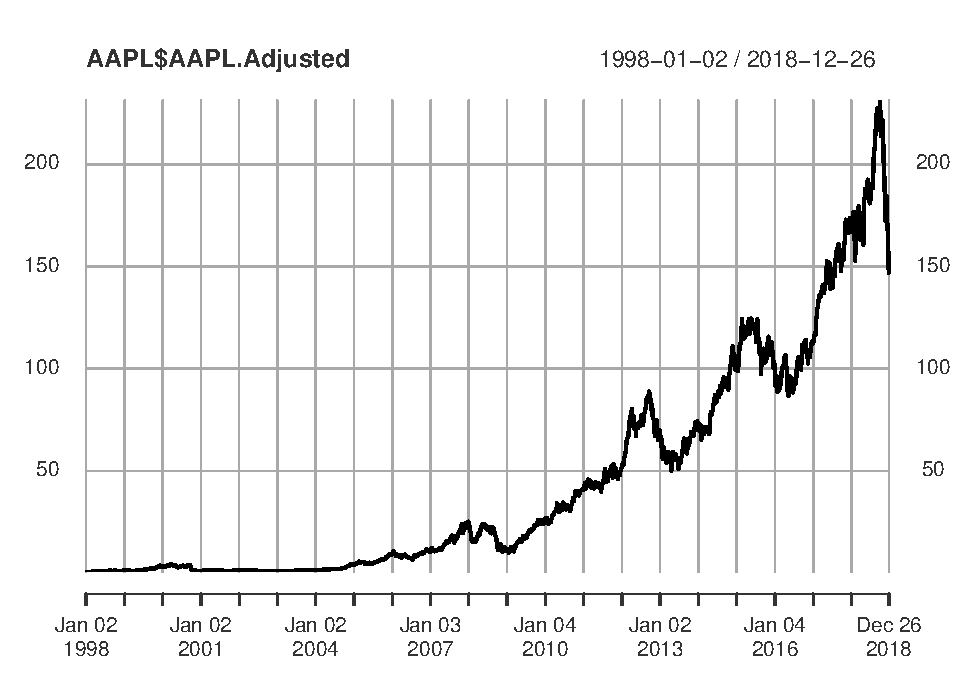
\includegraphics{open-quant-live-book_files/figure-latex/unnamed-chunk-9-1.pdf}

We called the \texttt{quantmod::getSymbols} function with the following
arguments:

\begin{itemize}
\tightlist
\item
  \texttt{Symbols=\textquotesingle{}AAPL\textquotesingle{}} defines a
  character vector specifying the names of each symbol to be loaded,
  here specified by the symbol of the company Apple Inc.;
\item
  \texttt{src="av"} specifies the sourcing method, here defined with the
  value corresponding to Alpha Vantage;
\item
  \texttt{output.size="full"}, strings \texttt{compact} and
  \texttt{full} are accepted with the following specifications:
  \texttt{compact} returns only the latest 100 data points;
  \texttt{full} returns the full-length time series of up to 20 years of
  historical data;
\item
  \texttt{adjusted=TRUE}, defines boolean variable to include a column
  of closing prices adjusted for dividends and splits;
\item
  \texttt{api.key}, specifies your Alpha Vantage API key.
\end{itemize}

\subsection{IEX}\label{iex}

\subsection{Quandl}\label{quandl}

\chapter{Stylized Facts}\label{stylized-facts}

\section{Introduction}\label{introduction}

\section{Distribution of Returns}\label{distribution-of-returns}

\subsection{Fat Tails}\label{fat-tails}

A distribuição de retornos financeiros apresenta leptokurtose. A
ocorrência de eventos extremos é mais provável comparado com uma
distribuição normal, i.e., as caudas da distribuição empírica de
retornos são mais ``pesadas'' comparadas com as caudas esperadas supondo
uma distribuição normal de probabilidade.

\subsection{Skewness}\label{skewness}

A distribuição empírica de retornos é distorcida para esquerda. Retornos
negativos são mais prováveis que retornos positivos.

\section{Volatility}\label{volatility}

\begin{equation}
 \sigma = \sqrt{ \frac{1}{N-1} \sum_{i=1}^N (x_i - \overline{x})^2}
\label{eq:sd}
\end{equation}

\subsection{Time-invariance}\label{time-invariance}

A volatilidade de retornos financeiros não é constante ao longo do
tempo.

\subsection{Volatility Clustering}\label{volatility-clustering}

Eventos extremos são observados próximos um dos outros.

\subsection{Correlation with Trading
Volume}\label{correlation-with-trading-volume}

O volume de negociação de um ativo tem correlação significante com a
volatilidade do mesmo.

\section{Correlation}\label{correlation}

\begin{equation}
\label{eq:correlation}
\rho = \frac{\sum\limits_{t=1}^{T} (r_t - \hat{r}_t)(s_t - \hat{s}_t)}{\sqrt{\sum\limits_{t=1}^{T} (r_t^{\tau} - \hat{r}_t^{\tau})^2}\sqrt{\sum\limits_{t=1}^{T}(s_t - \hat{s}_t)^2}},
\end{equation}

onde \(\hat{r}_t\) e \(\hat{s}_t\) são a média amostral de \(r_t\) e
\(s_t\), respectivamente.

\subsection{Time-invariance}\label{time-invariance-1}

A correlação entre duas series temporais de retornos financeiros não é
constante ao longo do tempo.

\subsection{Auto-correlation}\label{auto-correlation}

Retornos financeiros apresentam baixa autocorrelação (linear), exceto em
escalas de tempo muito baixas, e.g., minutos, onde há presença de
efeitos de microstructura. Por outro lado, a função de autocorrelação do
valor absoluto de retornos financeiros decai lentamente com o tempo.

A correlação contemporânea é maior do que a correlação cruzada.

\chapter{Correlation \& Causation}\label{correlation-causation}

\part{Algo Trading}\label{part-algo-trading}

\chapter{Limit Order}\label{limit-order}

\part{Portfolio
Optimization}\label{part-portfolio-optimization}

\part{Machine Learning}\label{part-machine-learning}

\part{Econophysics}\label{part-econophysics}

\chapter{Entropy}\label{entropy}

\chapter{Transfer Entropy}\label{transfer-entropy}

\chapter{Financial Networks}\label{financial-networks}

\bibliography{book.bib,packages.bib}

\end{document}
